\documentclass[english,russian,a4paper,12pt]{article}
\usepackage[utf8]{inputenc}
\usepackage[T2A]{fontenc}
\usepackage{babel}
\usepackage{csquotes}

\usepackage{fullpage}
\usepackage{indentfirst}
\usepackage[font=small,labelfont=bf,labelsep=period]{caption}
\usepackage{graphicx}
\usepackage{wrapfig}
\usepackage{subcaption}
\usepackage{paralist}

\usepackage{amssymb, amsmath}

\usepackage{tikz}
\usetikzlibrary{arrows,fit,positioning,shapes.multipart}

\usepackage[
	pdfauthor={Oleg Rogozin},
	pdftitle={Ghost effect between two parallel plates},
	colorlinks,pdftex, unicode]{hyperref}

\newcommand{\Kn}{\mathrm{Kn}}
\newcommand{\dd}{\:\mathrm{d}}
\newcommand{\pder}[2][]{\frac{\partial#1}{\partial#2}}
\newcommand{\pderder}[2][]{\frac{\partial^2 #1}{\partial #2^2}}

\begin{document}

\tableofcontents

\section{Введение}

Для описания жидкости и газа в общем виде используются уравнения сохранения массы, импульса и энергии:
\begin{gather}
	\pder[\rho]{t} + \pder{x_i}(\rho v_i) = 0, \label{eq:mass}\\
	\pder{t}(\rho v_i) + \pder{x_j}(\rho v_i v_j + p_{ij}) = \rho F_i, \label{eq:momentum}\\
	\pder{t}\left[\rho\left(e+\frac{v_i^2}2\right)\right] +
		\pder{x_j}\left[\rho v_j\left(e+\frac{v_i^2}2\right)+v_i p_{ij}+q_j\right] = \rho v_j F_j. \label{eq:energy}
\end{gather}
Макроскопические параметры: \(\rho\) "--- плотность, \(v_i\) "--- скорость, \(p_{ij}\) "--- тензор напряжений,
\(e\) "--- удельная внутренняя энергия, \(q_i\) "--- тепловой поток. \(F_i\) "--- внешняя сила.
Для идеального одноатомного газа внутренняя энергия~\(e\) зависит только от температуры~\(T\):
\[ e = \frac32RT,\]
где \(R=k_B/m\) "--- удельная газовая постоянная. Давление выражается через уравнение состояния:
\[ p = \rho RT. \]

Для замыкания уравнений сохранения~\eqref{eq:mass}--\eqref{eq:energy}
необходимо определить тензор напряжений \(p_{ij}\) и поток тепла \(q_i\).
В классической гидрогазодинамике используется так называемая навье"--~стоксовкая система уравнений:
\begin{gather}
	p_{ij} = p\delta_{ij} - \mu\left(\pder[v_i]{x_j}+\pder[v_j]{x_i}-\frac23\pder[v_k]{x_k}\delta_{ij}\right) -
		\mu_B\pder[v_k]{x_k}\delta_{ij}, \label{eq:stress_tensor}\\
	q_i = -\lambda\pder[T]{x_i}. \label{eq:heat_flow}
\end{gather}
Здесь \(\mu\) "--- вязкость, \(\mu_B\) "--- вторая вязкость, \(\lambda\) "--- теплопроводность. 

Линейные соотношения~\eqref{eq:stress_tensor}--\eqref{eq:heat_flow} называются
также законами Ньютона и Фурье соответственно.
Изначально они имели феменологический характер, позже были получены с помощью разложения Чепмена"--~Энскога
из уравнения Больцмана в предположении малости градиентов макропараметров:
\[ \frac{|\nabla h|}{h}\ell = o(1), \quad h = \{\rho, T, v_i\}, \]
где \(\ell\) "--- это длина свободного пробега,
зависящая от радиуса действия межмолекулярного потенциала взаимодействия \(d_m\)
(для модели твёрдых сфер это просто диаметр):
\begin{equation}
	\ell = \frac{m}{\sqrt2\pi d_m^2 \rho}.
\end{equation}

В общем случае необходимо учитывать нелинейные члены в выражении для тензора напряжений \(p_{ij}\) и теплового потока \(q_i\).
В данной работе будем уделять внимание только уравнению теплопроводности.

\section{Асимптотический анализ уравнения Больцмана}
Подробный математический вывод [Бобылев 1996] приведённых ниже результатов можно найти в [Sone].

Стационарное уравнение Больцмана в отсутствии внешних сил в безразмерных переменных имеет вид:
\begin{equation}\label{eq:Boltzmann}
	\xi_i\pder[f]{x_i} = \frac1k J(f,f),
\end{equation}
\begin{equation}\label{eq:integral}
	J(f,g) = \frac12 \int(f'g'_*+g'f'_*-fg_*-gf_*)B\dd\Omega(\boldsymbol\alpha)\dd \boldsymbol\xi_*,
\end{equation}
где \(\Omega(\boldsymbol{\alpha})\) "--- телесный угол единичного вектора \(\boldsymbol\alpha\),
\(B\) "--- функционал межмолекулярного потенциала.
\[ k = \frac{\sqrt\pi}2\Kn, \quad \Kn = \frac{\ell}L. \]
Число Кнудсена \(\Kn\) определяет отношение длины свободного пробега \(\ell\) к характерному размеру задачи \(L\).

Функция распределения \(f(x_i,\xi_i)\) раскладывается в ряд по \(k\)
\[ f = f_0 + f_1k + f_2k^2 + \cdots \]
следующим образом:
\begin{align*}
	J(f_0,f_0) &= 0, \\
	2J(f_0,f_m) &= \xi_i\pder[f_{m-1}]{x_i} - \sum\limits_{r=1}^{m-1}J(f_r,f_{m-r}), \quad m \in \mathbb{N}.
\end{align*}
Такое разложение впервые предложил Гильберт [1911]. Далее будем использовать дополнительное условие
\[ \int\xi_if\dd\xi = O(k), \]
означающее, что число Маха такого же порядка малости, что и число Кнудсена.

Макропараметры также разложим по числу Кнудсена:
\[ h = h_0 + h_1k + h_2k^2 + \cdots. \]

Конечным результатом анализа является следующая система уравнений для \(T_0\), \(v_{i1}\), \(p_2\)
на основе модели твёрдых сфер:
\begin{align}
	\pder{x_i}(\rho_0v_{i1}) &= 0, \label{eq:asymptotic1} \\
	\rho_0v_{j1}\pder[v_{i1}]{x_j} &= -\frac12\pder[p_2^\dag]{x_i} \notag\\
		&+ \frac12\pder{x_j}\left[\gamma_1\sqrt{T_0}\left(
			\pder[v_{1i}]{x_j}+\pder[v_{1j}]{x_i}-\frac23\pder[v_{1k}]{x_k}\delta_{ij}\right
		)\right] \notag\\
		&+ \gamma_7\pder[T_0]{x_i}\pder[T_0]{x_j}\left(
			\frac{u_{1j}}{\gamma_2T_0\sqrt{T_0}} + \frac{T_0}4\pder[T_0]{x_j}
		\right), \label{eq:asymptotic2} \\
	\rho_0v_{i1}\pder[T_0]{x_i} &= \frac{\gamma_2}2\pder{x_i}\left(
		\sqrt{T_0}\pder[T_0]{x_i}
	\right). \label{eq:asymptotic3}
\end{align}
Давления \(p_0\), \(p_1\) являются константами,
\[ 
	p_2^\dag = p_2 + 
		\frac{2\gamma_3}{3p_0}\pder{x_k}\left(T_0\pder[T_0]{x_k}\right) -
		\frac{\gamma_7}{6p_0}\left(\pder[T_0]{x_k}\right)^2,
\]
\[ \rho_0 = \frac{p_0}{T_0}. \]

Для модели твёрдых сфер безразмерные коэффициенты переноса равны
\begin{alignat*}{2}
	\gamma_1 &= 1.270042427, &\quad \gamma_2 &= 1.922284066, \\
	\gamma_3 &= 1.947906335, &\quad \gamma_7 &= 1.758705.
\end{alignat*}

Граничные условия на границе с диффузным отражением имеют вид:
\begin{gather}
	T_0 = T_{w0}, \\
	\left\{
	\begin{aligned}
		& \frac{(v_{j1}-v_{wj1})(\delta_{ij}-n_jn_i)}{\sqrt{T_{w0}}} = 
			-\frac{K_1}{p_0}\pder[T_0]{x_j}(\delta_{ij}-n_jn_i), \\
		& v_{j1}n_j = 0.
	\end{aligned}
	\right.
\end{gather}
Здесь \(n_i\) "--- нормаль к поверхности, \(v_{wj1}\), \(T_{w0}\) "--- скорость и температура границы.
\(K_1\) "--- безразмерный коэффициент температурного скачка. Для модели твёрдых сфер 
\[ K_1 = -0.6463. \]

\subsection{Эффект призрака}

Из системы \eqref{eq:asymptotic1}--\eqref{eq:asymptotic3} видно, что в гидродинамическом пределе (при \(\Kn\to0\))
газ в общем случае не описывается уравнением Фурье.
На распределение температуры \(T=T_0\) влияет член скорости первого порядка малости \(v_{i1}\).
Таким образом, \(v_{i1}\) инфинитезимальным образом влияет на само поле скоростей \(v_i\),
но конечным на поле температуры.
Данная особенность асимптотического решения называется эффектом призрака [Соне].

Сходимость к уравнению Фурье наблюдается только в частном случае при \(v_{i1} = 0\).
Это возможно только при параллельности изотермических поверхностей:
\begin{equation}
	e_{ijk}\pder[T_0]{x_j}\pder{x_k}\left(\pder[T_0]{x_l}\right)^2 = 0.
\end{equation}

\section{Постановка задачи}

\begin{wrapfigure}{r}{7.4cm}
	\vspace{-10pt}
	\centering
	\usetikzlibrary{decorations.pathreplacing}
	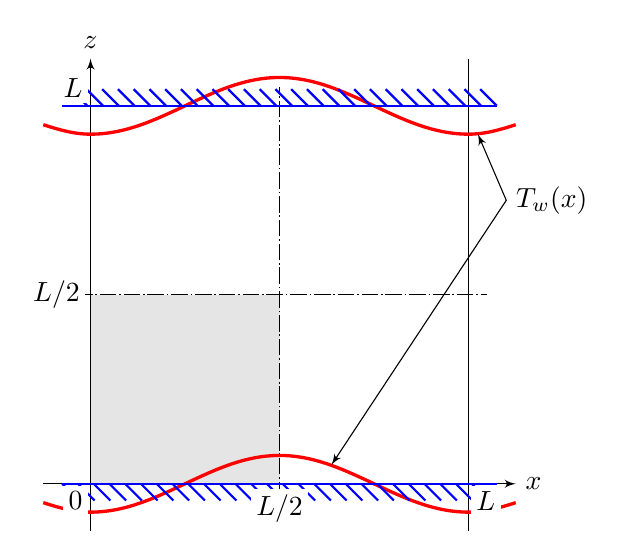
\begin{tikzpicture}[dashdot/.style={dash pattern=on .6pt off 1pt on 6pt off 1pt},
				interface/.style={postaction={draw, decorate, decoration=
					{border, angle=-45, amplitude=0.3cm, segment length=2mm}}},
				label/.style={fill=white, inner sep=2pt},
				>=latex', scale=1.2]
		\fill[gray!20] (0,0) -- (2,0) -- (2,2) -- (0,2) -- cycle;
		\draw[->] (-.5,0) -- (4.5,0) node[right] {\(x\)};
		\draw[->](0,-.5) -- (0,4.5) node[above] {\(z\)};
		\draw(4,-.5) -- (4,4.5);
		\draw[dashdot] (-.2,2) -- (4.2,2);
		\draw[dashdot] (2,-.2) -- (2,4.2);
		\draw[red, very thick] (-.5,-.2) sin (0,-.3) cos (1,0) sin (2,.3) cos (3,0) sin (4,-.3) cos (4.5,-.2);
		\draw[red, very thick] (-.5,3.8) sin  (0,3.7) cos (1,4) sin (2,4.3) cos (3,4) sin (4,3.7) cos (4.5,3.8);
		\draw[blue, thick, interface](-.3,0) -- (4.3,0);
		\draw[blue, thick, interface](4.3,4) -- (-0.3,4);
		\draw[<->] (4.1,3.7) -- (4.4,3) node[right] {\(T_w(x)\)} -- (2.55,.2);
		\node at (-.02,-.02) [below left, label] {0};
		\node at (4.02,-.02) [below right, label] {\(L\)};
		\node at (-.02,4.02) [above left, label] {\(L\)};
		\node at (-.05,2) [left, label] {\(L/2\)};
		\node at (2,-.05) [below, label] {\(L/2\)};
	\end{tikzpicture}
	\vspace{-15pt}
	\caption{Геометрия задачи.}\label{pic:geometry}
	\vspace{-5pt}
\end{wrapfigure}

Рассмотрим плоскую периодическую геометрию, как на рис.~\ref{pic:geometry}.
Газ расположен между двумя покоющимися (\(u_{wi} = 0\)) бесконечными параллельными пластинами,
разделённых на расстояние \(L\). Температура распределена на них по синусоидальному закону:
\begin{equation}
	T_w = 1-\alpha\cos{\frac{2\pi x}L}.
\end{equation}

В силу симметрии задачи расчётная область представляет собой квадрат со стороной \(L/2\).
На рисунке выделена серым цветом.

Интерес представляет сравнение температурных полей, полученных на основе уравнения Фурье и кинетической теории.
С помощью прямого численного моделирования уравнения Больцмана проанализируем сходимость решения для малых \(\Kn\).

Столкновения молекул газа описывается моделью твёрдых сфер. От пластин происходит полное диффузное отражение. 

\section{Решение задачи в гидродинамическом пределе}

В классической газовой динамике поставленная задача описывается простым уравнением теплопроводности:
\begin{equation}\label{eq:classic_solution}
	\pder{x_i}\left(\sqrt{T}\pder[T]{x_i}\right) = 0.
\end{equation}
Здесь учтено, что теплопроводность идеального одноатомного газа, состоящего из твёрдых сфер,
пропорциональна \(\sqrt{T}\).
 
Граничные условия на твёрдой стенке:
\[ T = T_w, \]
на плоскостях симметрии:
\[ \pder[T]{x_i}n_i = 0. \]

Точное решение, получаемое асимптотически из уравнения Больцмана (\eqref{eq:asymptotic1}--\eqref{eq:asymptotic3})
в пределе \(\Kn \to 0\), выражается системой:
\begin{align*}
        \pder[v_{i1}]{x_i}T &= v_{i1}\pder[T]{x_i}, \\
        e_{lmi}\pder{x_m}\left\{
		\frac{v_{j1}}{T}\pder[v_{i1}]{x_j}
		\right.&- \frac{\gamma_1}2\pder{x_j}\left[\sqrt{T}\left(\pder[v_{1i}]{x_j}+\pder[v_{1j}]{x_i}-\frac23\pder[v_{1k}]{x_k}\delta_{ij}\right)\right] \\
		&-\left. \gamma_7\pder[T]{x_i}\pder[T]{x_j}\left(\frac{u_{1j}}{\gamma_2T\sqrt{T}} + \frac{T}4\pder[T]{x_j} \right)
	\right\} = 0, \\
        v_{i1}\pder[T]{x_i} &= \frac{\gamma_2}4\sqrt{T}\left[\left(\pder[T]{x_i}\right)^2 + T\pderder[T]{x_i}\right].
\end{align*}
Ротор от~\eqref{eq:asymptotic2} позволяет избавиться от \(p_2^\dag\).
Для простоты константное давление \(p_0\) взято единичным:
\[ p = p_0 = 1. \]
Индекс у температуры \(T\) исчез, поскольку при \(k=0\) получается точное равенство \(T=T_0\).

\section{Решение для произвольных чисел Кнудсена}

\section{Сравнение результатов}

\end{document}


